\documentclass[a4paper, 11pt]{article}
\usepackage[english]{babel}
% \usepackage[top=2cm,bottom=2cm,left=2cm,right=2cm]{geometry}
\usepackage[utf8]{inputenc}
\usepackage{import}
\usepackage{float}
\usepackage{subfigure}
% \usepackage{subfig}
\usepackage[pdftex]{graphicx}
% \usepackage{graphicx}
\usepackage{amssymb,amsmath,amsthm,amsfonts}
\usepackage{xspace}
\usepackage{tabularx}
\usepackage{indentfirst}
\usepackage{wrapfig,booktabs}
%\usepackage[small]{caption}
% \usepackage{subcaption}
\usepackage{eucal}
\usepackage{eso-pic}
\usepackage{hyperref}
\usepackage{url}
\usepackage{booktabs}
\usepackage{afterpage}
\usepackage{parskip}
\usepackage{listings}
\usepackage{fancyhdr}
\usepackage{textcomp}
\usepackage{cite}
\usepackage{multirow,multicol}
\usepackage{setspace}
\usepackage[version=4]{mhchem}
\usepackage{nicefrac}
\usepackage{siunitx}

\usepackage{caption}
\captionsetup{tableposition=top,font=small,width=0.8\textwidth}
%\usepackage[table]{xcolor}
\usepackage[arrowdel]{physics}
\usepackage{mathtools}
\usepackage{tablefootnote}
\usepackage{enumitem}

\setlist[description]{font={\scshape}} %style=unboxed,style=nextline
\usepackage{floatflt}
\usepackage{commath}
\usepackage{bm}
\usepackage{ifthen}
\usepackage{comment}
\usepackage[colorinlistoftodos,textsize=tiny]{todonotes}

\newcommand{\overbar}[1]{\mkern 1.5mu\overline{\mkern-1.5mu#1\mkern-1.5mu}\mkern 1.5mu}
\let\oldfrac\frac
\renewcommand{\frac}[3][d]{\ifthenelse{\equal{#1}{d}}{\oldfrac{#2}{#3}}{\nicefrac{#2}{#3}}}

\usepackage[top=2cm,bottom=2cm,left=2cm,right=2cm]{geometry}
\usepackage[utf8]{inputenc}
\usepackage{import}
\usepackage{float}
\usepackage{subfigure}
% \usepackage{subfig}
\usepackage[pdftex]{graphicx}
% \usepackage{graphicx}
\usepackage{amssymb,amsmath,amsthm,amsfonts}
\usepackage{xspace}
\usepackage{tabularx}
\usepackage{indentfirst}
\usepackage{wrapfig,booktabs}
%\usepackage[small]{caption}
% \usepackage{subcaption}
\usepackage{eucal}
\usepackage{eso-pic}
\usepackage{hyperref}
\usepackage{url}
\usepackage{booktabs}
\usepackage{afterpage}
\usepackage{parskip}
\usepackage{listings}
\usepackage{fancyhdr}
\usepackage{textcomp}
\usepackage{cite}
\usepackage{multirow,multicol}
\usepackage{setspace}
\usepackage[version=4]{mhchem}
\usepackage{nicefrac}
\usepackage{siunitx}

\usepackage{caption}
\captionsetup{tableposition=top,font=small,width=0.8\textwidth}
%\usepackage[table]{xcolor}
\usepackage[arrowdel]{physics}
\usepackage{mathtools}
\usepackage{tablefootnote}
\usepackage{enumitem}

\setlist[description]{font={\scshape}} %style=unboxed,style=nextline
\usepackage{floatflt}
\usepackage{commath}
\usepackage{bm}
\usepackage{ifthen}
\usepackage{comment}
\usepackage[colorinlistoftodos,textsize=tiny]{todonotes}

\newcommand{\overbar}[1]{\mkern 1.5mu\overline{\mkern-1.5mu#1\mkern-1.5mu}\mkern 1.5mu}
\let\oldfrac\frac
\renewcommand{\frac}[3][d]{\ifthenelse{\equal{#1}{d}}{\oldfrac{#2}{#3}}{\nicefrac{#2}{#3}}}


\begin{document}

\title{Montecarlo simulations on the D-dimensional Ising model}
\author{Alessandro Lovo}

\maketitle


\section{Introduction}
  The aim of this report is to use Montecarlo (MC) simulations to study the paramagnetic-ferromagnetic phase transition of an Ising model as a function of dimension $D$ and of the size of the system. Some ways of optimizing the simulations will also be discussed.

  \subsection{Setting up the model}
    An Ising model is a description of a magnetic system via a set of \emph{spins} interacting with each other.
    There are many variaions on the theme of the Ising model, but here the focus is on the most commonly used, i.e. the one where each spin $S_i \in \{-1, +1\}$, spins are arranged in a $D$ dimensional simple cubic lattice and each spin interacts only with its nearest neighbors ($n.n.$).
    The number of nearest neighbors per spin is defined as the coordination number $z = 2D$

    The hamiltonian of the system can then be written as

    \begin{equation*}
      H = -\frac{1}{2} J \sum_i \sum_{j \, n.n. \, i} S_i S_j - B \sum_i S_i
    \end{equation*}

    where $J$ is the coupling constant between spins and $B$ is the external uniform magnetic field to which spins tend to align. However since the system will be in thermal equilibrium at temperature $T$ is is enough to consider the reduced energy

    \begin{equation*}
      E = \frac{H}{k_BT} = -\frac{J}{2k_BT}  \sum_i \sum_{j \, n.n. \, i} S_i S_j - \frac{B}{k_BT} \sum_i S_i = -k\sum_i \sum_{j \, n.n. \, i} S_i S_j - h\sum_i S_i
    \end{equation*}

    Since the system has finite size one should deal with its surface: concerning this one could consider three possible boundary conditions:
    \begin{itemize}
      \item \emph{free}, where the system is surrounded by a layer of spins with value fixed to $0$
      \item \emph{fixed}, where the system is surrounded by a layer of spins with value fixed to $+1$ or $-1$
      \item \emph{periodic}, where the system is surrounded by a layer of spins that 'mirrors' the opposite surface as if the system was periodically replicated.
    \end{itemize}
    The most used one will be the periodic boundary condition, but the others will be interesting when investigating size dependent properties.

    At this point, if the system has $N$ spins, one can define some useful quantities to be monitored during the simulations:
    \begin{itemize}
      \item magnetization per spin $m = \frac{1}{N} \sum_i S_i \in [-1, 1]$
      \item degree of alignment per spin $a = \frac{1}{zN} \sum_i \sum_{j \, n.n. \, i} S_i S_j \in [-1, 1]$ that if $h = 0$ is equal to $-\frac{E}{kNz} = -\frac{2H}{J}$
      % \item density of domain walls $n_{DW} = \frac{N_{DW}}{N} = \frac{N - N_{sat}}{N}$ where $N_{sat}$ is the number of \emph{saturated} spins, i.e. spins that have the same value of all their nearest neighbors
    \end{itemize}

    By combining the results of different simulations one can then compute the two response functions:
    \begin{itemize}
      \item specific heat at constant external field $\frac{1}{N} \frac{\partial \langle H \rangle }{\partial T} \propto -\frac{\partial \langle a \rangle }{\partial \frac[f]{1}{k}} =: c_B$
      \item magnetic susceptibility $\frac{\partial N|m|}{\partial H} = \frac{1}{Nk_BT} \text{Var}(N|m|) \propto Nk(\langle m^2 \rangle - \langle |m| \rangle^2 ) =: \chi_m$ \footnote{In theory the magnetic susceptibility should be defined in terms of $m$ and not $|m|$, but for finite size systems the latter works better (see \cite{rif:eye-opener} pag 15).}
    \end{itemize}

    % The advantage of using this quantities is that $m,a \in [-1,1]$ independently on the parameters of the system $N,D,k,h$ making them suitable to be studied on a wide range of those parameters.

  \subsection{Montecarlo evolution of the system}
    After deciding an initial configuration of the system, at each MC step one attempts to make a \emph{move} and then computes the variation of the reduced energy $\Delta E$. If $\Delta E < 0$ the move is accepded. Otherwise a random number $r \in [0,1)$ is extracted and if $r < e^{-\Delta E}$ the move is accepted as well. If the move is rejected the system stays in its original configuration.
    One has now to decide a proper move, and in principle one could say 'pick $n$ spins and flip them' where 'pick' can be done by choosing them randomly or by cycling with some order amongst all spins.

    After a large enough number of MC steps the system should reach equilibrium and at this point one can collect meanigful data to analyze.


  \section{Choice of the simulation parameters}
    Henceforth, if not otherwise specified, simulations will be run with periodic boundary condition and $h = 0$. \\
    To obtain meanigful results in a reasonable amount of time it is necessary to optimize the simulation parameters. In this section a 2-dimensional Ising model with $128 \times 128$ (this way it is easy to visualize the system as a black and white picture) spins will be used to test the effect of the various simulation parameters.


    \subsection{How to 'pick' spins}
      Suppose for now that $n = 1$, i.e. at each step one flips a single spin. In order to see what is the difference between randomly picking a spin versus cycling them one can initialize the system with random noise and then do $10^7$ MC steps with a very high value of the coupling constant between spins $k = 8$. This way one expects the system to reach a ferromagnetic equilibrium state.

      \begin{figure}[H]
        \centering
        \resizebox{0.45\textwidth}{!}{\import{img/}{m_k16_random.pgf}} \quad
        \resizebox{0.45\textwidth}{!}{\import{img/}{m_k16_permutate_c1.pgf}}
        \caption{Behavior of the magnetization of the system along 5 trials. The first is in the case of random picking, the second cycling. One of the final configurations for each type of picking is reported in fig \ref{fig:fin_na}, \ref{fig:fin_nc}.}
        \label{fig:pick_m}
      \end{figure}

      In fig \ref{fig:pick_m} it is clear that cycling the spins instead of randomly picking them allows to reach the equilibrium state much faster. This can be explained by considering that when cycling the spins after $128^2 \approx 1.6\cdot10^4$ steps all spins had the opportunity to flip. On the other hand with the random picking it takes on average $128^2 \ln (128^2) \approx 1.6\cdot10^5$ steps before that hapens. This discrepancy increases if one considers the number of steps after which every spin had the opportunity to flip $M$ times.\\
      In order to avoid correlation in the spins, a nice way of cycling is to randomly permute the sequence of indices of the spins $\{i\}_{i=1}^N$ and then pick them following the permuted sequence $\{i_j\}_{j=1}^N$.

    \subsection{How many spins to pick}
      First of all one should notice that picking together $n > 1$ spins is incompatible with the cycling technique as the $n$-uples of spins will periodically repeat somehow partitioning the system in groups. And actually in this case the system does not evolve at all (fig \ref{fig:fin_nb}).
      On the other hand with random picking the correlation introduced is much lower and the system is still able to evolve although slower (fig \ref{fig:fin_nc}, \ref{fig:fin_nd}). For this reason it is better to use $n = 1$.

      \begin{figure}
        \centering
        \begin{subfigure}[]{
          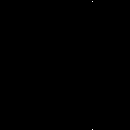
\includegraphics[width=0.2\textwidth]{img/k16_cycle_j37_fin_c1.png}
          \label{fig:fin_na}}
        \end{subfigure}
        \begin{subfigure}[]{
          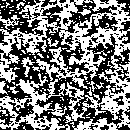
\includegraphics[width=0.2\textwidth]{img/k16_cycle_j37_fin_c2.png}
          \label{fig:fin_nb}}
        \end{subfigure}
        \begin{subfigure}[]{
          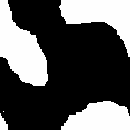
\includegraphics[width=0.2\textwidth]{img/k16_random_fin.png}
          \label{fig:fin_nc}}
        \end{subfigure}
        \begin{subfigure}[]{
          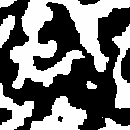
\includegraphics[width=0.2\textwidth]{img/k16_random_fin_c2.png}
          \label{fig:fin_nd}}
        \end{subfigure}
        \caption{Final configuration after $10^7$ steps starting from random noise done for $n = 1$, cycling (a); $n = 2$, cycling (b); $n = 1$, random (c) and $n = 2$, random (d).}
      \end{figure}



      % \subsection{Reasonable values for $k$}
      %   Since the idea is to simulate at different values of $k$ and hopefully see a phase transition it is useful to make some rough estimations in order to look in the correct range of $k$s.\\
      %   If one considers the perfectly ferromagnetic configuration in which all the spins are aligned the probability of one of them flipping is $p_1 = e^{-\Delta E} = e^{-2kz}$.
      %   So, if one calls $N_{s}$ the number of spins not aligned with all the rest (henceforth 'seed' spins) and if $N_{s} \ll N$ one can write the following differential equation noting that if a seed spin is picked, it flips with probability 1.
      %
      %   \begin{equation}
      %     \frac{\partial N_{s}}{\partial t} = p_1\frac{N - N_{s}}{N} - \frac{N_{s}}{N} = p_1 - \frac{1}{N}(1 + p_1) N_s
      %   \end{equation}
      %
      %   Starting from $N_s(0) = 0$, the above equation has solution
      %
      %   \begin{equation}
      %     N_{s}(t) = \frac{p_1N}{1 + p_1}\left(1 - e^{-\frac{p_1 + 1}{N}t}  \right) \xrightarrow[t \to \infty]{} \frac{p_1N}{1 + p_1}
      %   \end{equation}
      %
      %   If now one supposes $\frac{N_s}{N} < r$, this implies $p_1 < \frac{r}{1 - r}$ and thus $k > \frac{1}{2z} \ln(\frac{1 - r}{r})$. For the square lattice ($z = 4$) one gets  $\frac{N_s}{N} < 0.001$ if $k > 0.86$.
      %
      %   With a more sophisticated reasoning one can consider that the flipping probability of a spin next to a seed is $p_2 = e^{-\Delta E} = e^{-2k(z-2)}$ and this time the differential equation for $N_s$ becomes
      %
      %   \begin{equation}
      %     \frac{\partial N_{s}}{\partial t} = p_1\frac{N - N_{s}}{N}  + p_2 \frac{zN_s}{N}- \frac{N_{s}}{N} = p_1 - \frac{1}{N}(1 + p_1 - zp_2) N_s
      %   \end{equation}
      %
      %   The big difference is that now $1 + p_1 - zp_2$ can be smaller than 0 yielding an exponential increase of the number of seeds and thus the transition to the paramagnetic state. The condition for the transition $1 + p_1 - zp_2 < 0$ can be recasted as $ze^{4k} > e^{2zk} + 1$ and then solved graphically.
      %   If one denotes as $k_l$ the threshold values obtained this way and $k_u$ the ones obtained by the previous reasoning, namely, $k_u$ is the value of $k$ at which one expects a $0.1\%$ fraction of seeds, one gets the results in tab \ref{tab:k_crit_th}.
      %   a reasonable range for the choice of the $k$ points could be $[\frac{k_l}{2}, k_u]$. In the case $D = 1$ the lowest value of $k$ can be arbitrarily chosen to be $0.5$.
      %   It is interesting to notice that in $D = 1$ the ferromagnetic state is always unstable, i.e. there is no phase transition, in agreement with statistical mechanics predictions. Moreover Onsanger's exact solution of the 2-dimensional Ising model predicts $k_{c}^{exact} = \frac{\ln(1 + \sqrt{2})}{4} \approx 0.22$. which is not very far from the value predicted by this very rough reasoning.
      %
      %   \begin{table}[H]
      %     \centering
      %     \begin{tabular}{cccccccc}
      %       \toprule
      %       $D$ & $z$ & $k_l$ & $k_u$ \\
      %       \midrule
      %       $1$ & $2$ & $ < 0$ & $1.73$ \\
      %       $2$ & $4$ & $0.33$ & $0.86$ \\
      %       $3$ & $6$ & $0.22$ & $0.57$ \\
      %       $4$ & $8$ & $0.17$ & $0.43$ \\
      %       \bottomrule
      %     \end{tabular}
      %     \caption{Critical value of $k$ from this simple model of the instability of the ferromagnetic saturated}
      %     \label{tab:k_crit_th}
      %   \end{table}
      %
      %   If one denotes as $k_l$ the threshold values in tab \ref{tab:k_crit_th} and $k_u$ the ones obtained by the previous reasoning, namely, $k_u$ is the value of $k$ at which one expects a $0.1\%$ fraction of seeds, a reasonable range for the choice of the $k$ points could be $[\frac{k_l}{2}, k_u]$. In the case $D = 1$ the lowest value of $k$ can be arbitrarily chosen to be $0.5$.


    \subsection{Reasonable values for $k$}
      Since the idea is to simulate at different values of $k$ and hopefully see a phase transition it is useful to make some rough estimations in order to look in the correct range of $k$s.\\
      If one considers the perfectly ferromagnetic configuration in which all the spins are aligned the probability of one of them flipping is $p_1 = e^{-\Delta E} = e^{-4kz}$.
      On the other hand the flipping probability of a spin next to an already fliped spin is $p_2 = e^{-\Delta E} = e^{-4k(z-2)}$.
      So, if one calls $N_{s}$ the number of spins not aligned with all the rest (henceforth 'seed' spins) and if $N_{s} \ll N$ one can write the following differential equation noting that if a seed spin is picked, it flips back with probability 1.

      \begin{equation*}
        \frac{\partial N_{s}}{\partial t} = p_1\frac{N - N_{s}}{N}  + p_2 \frac{zN_s}{N}- \frac{N_{s}}{N} = p_1 - \frac{1}{N}(1 + p_1 - zp_2) N_s
      \end{equation*}

      Starting from $N_s(0) = 0$, the above equation has solution

      \begin{equation*}
        N_{s}(t) = \frac{p_1N}{1 + p_1 - zp_2}\left(1 - e^{-\frac{1 + p_1 -zp_2}{N}t}  \right)
      \end{equation*}

      Now $1 + p_1 - zp_2$ can be smaller than 0 yielding an exponential increase of the number of seeds and thus the transition to the paramagnetic state. The condition for the transition $1 + p_1 - zp_2 < 0$ can be recasted as $ze^{8k} > e^{4zk} + 1$ and then solved graphically finding the lower threshold values of $k_l$ in tab \ref{tab:k_crit_th}.
      It is interesting to notice that in $D = 1$, $p_2 = 1$ and thus $1 + p_1 - zp_2 < 0 \, \forall k > 0$, meaning that the ferromagnetic state is always unstable, i.e. there is no phase transition, in agreement with statistical mechanics predictions. Moreover Onsanger's exact solution of the 2-dimensional Ising model predicts $k_{c}^{exact} = \frac{\ln(1 + \sqrt{2})}{4} \approx 0.22$. which is not very far from the value predicted by this very rough reasoning ($k_l = 0.17$).
      On the other hand if $1 + p_1 - zp_2 > 0$, $N_s(t) \xrightarrow[t \to \infty]{} \frac{p_1N}{1 + p_1 - zp_2} \approx \frac{p_1N}{1 - zp_2}$.
      If one sets a threshold $\frac{N_s(\infty)}{N} < 0.1\%$ one can graphically find the upper threshold values $k_u$ in tab \ref{tab:k_crit_th}.

      \begin{table}[H]
        \centering
        \begin{tabular}{cccccccc}
          \toprule
          $D$ & $z$ & $k_l$ & $k_u$ \\
          \midrule
          $2$ & $4$ & $0.17$ & $0.44$ \\
          $3$ & $6$ & $0.11$ & $0.29$ \\
          $4$ & $8$ & $0.09$ & $0.21$ \\
          \bottomrule
        \end{tabular}
        \caption{Threshold values for $k$ from this simple model of the instability of the ferromagnetic state.}
        \label{tab:k_crit_th}
      \end{table}

      Apart from the 1D case in which no phase transition is expected, for higher dimensions sudying the system in the range $[k_l,k_u]$ should be enough to visualize the phase transition. However, since these threshold values come from a pretty rough model, it is more conservative to use instead $[0.75k_l,1.25k_u]$.


    \subsection{Sampling rate, block averaging and lenght of the simulation}
      Since at each time step only a single spin has the opportunity to flip, a reasonable sampling rate is taking a snapshot of the system every $\tau_s \approx 10N$ steps: this way two subsequent snapshots should not be too much correlated. To further reduce this correlation and then be able to compute the error on the average properties of the system as the error of the arithmetic mean, one can proceed with the \emph{block averaging} technique, namely subdivide the set of sampled properties $\{f_i\}_{i=1}^n$ in $M$-uples of consecutive points and create a new dataset $\{f_j\}_{j=1}^{\frac[f]{n}{M}}$ made of the arithmetic mean of each $M$-ulpe.
      By monitoring how the standard deviation of the mean of the mean $\sigma(f) = \sqrt{\frac{\text{Var}\left( \{f_j\}_{j=1}^{\frac[f]{n}{M}} \right)}{\frac[f]{n}{M}}}$ varies with $M$ one finds that a proper value for the block averaging parameter is around $M = 100$ (fig \ref{fig:block_averaging}).
      Actually since with $\tau_s = 10N$ consecutive snapshots are still a lot correlated, rather than using $M = 100$ it is more computationally efficient to do $\tau_s = 50N$ and $M = 20$.

      % Also the magnetic susceptibility can be estimated as $\chi_m = Nk\sigma(m)^2$.

      At this point, after the block averaging process, points are spaced by $1000 N$ steps and in order to compute a meaningful average on these points (denoted with angular brakets) one should have at least around 20 of them, meaning that the simulation should last at least $2\cdot10^4 N$ timesteps.
      Since this numbers start to be quite big, to speed up the computations a $64\times64$ system will now be used.

      \begin{figure}[H]
        \centering
        \resizebox{0.5\textwidth}{!}{\import{img/}{block_averaging.pgf}}
        \caption{Behavior of the standard deviation of the mean magnetization as a function of the block averaging parameter $M$. $10^8$ step simulation run on a $64\times64$ Ising model at $k = 0.2$.}
        \label{fig:block_averaging}
      \end{figure}


    \subsection{Equilibration and initialization of the system}
      The equilibrium is reached in the first part of the simulation (equilibration), that should not be used for computing averages. In order to make this part as short as possible it is important to properly initialize the system (fig \ref{fig:equilibration}). One can notice that (unsurprisingly) a random noise configuration takes a while to reach the ferromagnetic equilibrium state, but on the other hand a ferromagnetic starting configuration reaches a paramagnetic equilibrium quite quickly.
      For this reason on can initialize the system with a ferromagnetic state and discard as equilibration the first two points after the block averaging process.

      \begin{figure}[H]
        \centering
        \resizebox{0.45\textwidth}{!}{\import{img/}{equilibration_k0.4_para.pgf}} \quad
        \resizebox{0.45\textwidth}{!}{\import{img/}{equilibration_k0.2_ferro.pgf}}
        \caption{Behavior of the magnetization with different initialization: the first one with starting from random noise at $k = 0.4$, the second starting from a ferromagnetic configuration at $k = 0.2$.}
        \label{fig:equilibration}
      \end{figure}



  \section{Results of the simulations}
    \subsection{$D = 1$}
      The one dimensional case is quite a tricky one: since one does not expect a phase transition the range of $k$ points is somewhat arbitrary. Here $[0.5,8]$ is used. For this large values of $k$, $p_1 \ll 1$, meaning that the probability of creating the first seed spin is almost negligible; but on the other hand $p_2 = 1$, and so as soon as there is one seed a wave of flipping spins will travel across the system, giving to the magnetization an 'instanton-like' behavior fig \ref{fig:instanton}. On the other hand if $k$ is big enough $p_1$ is so small that the system is stuck in the initial ferromagnetic configuration and so it doesn't evolve at all.

      \begin{figure}[H]
        \centering
        \resizebox{0.45\textwidth}{!}{\import{img/}{D1_N1024_k2.3_instanton.pgf}}
        \resizebox{0.45\textwidth}{!}{\import{img/}{D1_N1024_ferro_am.pgf}}
        \caption{Instanton-like behavior of the magnetization in a 1024 spin system at $k = 2.3$ and behavior of the magnetization and the average alignment as a function of $k$ when starting from the ferromagnetic phase and cycling spins.}
        \label{fig:instanton}
      \end{figure}

      To try to avoid this, one can istead start from the paramagnetic configuration (random noise) and use the random picking of spins. With this settings and trying for different sizes of the system one gets the results in fig \ref{fig:D1_size_dependent}, where it is clear that as the size of the system increases the ferromagnetic state becomes more and more unstable, suggesting that in the thermodynamic limit there is, as expected, no phase transition at all.

      \begin{figure}[H]
        \centering
        \resizebox{0.3\textwidth}{!}{\import{img/}{D1_N64_para_random_am.pgf}}
        \resizebox{0.3\textwidth}{!}{\import{img/}{D1_N256_para_random_am.pgf}}
        \resizebox{0.3\textwidth}{!}{\import{img/}{D1_N1024_para_random_am.pgf}}
        \caption{Behavior of the magnetization and the average alignment as a function of $k$ for three different sizes of the system starting from the paramagnetic phase and with random picking.}
        \label{fig:D1_size_dependent}
      \end{figure}


    \subsection{$D = 2$}
      In $D > 1$ one expects a phase transition at not too high values of $k$, meaning that the system shouldn't get stuck in the initial configuration. For this reason one can start from the ferromagnetic state and cycle the spins.

      By running the simulations at different sizes of the system one finds that the magnetization does exhibit a phase transition and moreover as $N$ increases the transition becomes sharper (fig \ref{fig:D2_size_dependent}), as expected since the system is getting closer to the thermodynamic limit.\\
      It is interesting here to try different boundary conditions: periodic (PBC) and free (FBC).
      If one plots the behavior of $a$ and $\chi_m$ (fig \ref{fig:D2_achi}) one finds that $a$ is almost unaffected by the size of the system with PBC while the free boundary data tend to the periodic ones as the size of the system increases. A similar behavior can be seen in the magnetic susceptibility, where basically the FBC exaggerates the effect of size.

      \begin{figure}[H]
        \centering
        \resizebox{0.3\textwidth}{!}{\import{img/}{D2_N8_am.pgf}}
        \resizebox{0.3\textwidth}{!}{\import{img/}{D2_N16_am.pgf}}
        \resizebox{0.3\textwidth}{!}{\import{img/}{D2_N64_am.pgf}}
        \caption{Behavior of the magnetization and the average alignment as a function of $k$ for three different sizes of the system (with PBC) starting from the ferromagnetic state and cycling spins.}
        \label{fig:D2_size_dependent}
      \end{figure}

      \begin{figure}
        \centering
        \resizebox{0.45\textwidth}{!}{\import{img/}{D2_a_free.pgf}}
        \resizebox{0.45\textwidth}{!}{\import{img/}{D2_chi_a.pgf}}
        \caption{Behavior of the average alignment and the of the magnetic susceptibility as a function of $k$ with different boundary conditions: solid line \emph{periodic}, dashed \emph{free}.}
        \label{fig:D2_achi}
      \end{figure}

      The magnetic susceptibility $\chi_m$ exhibits a peak whose maximum can be used to find the critical value of $k$ with error given by half of the full width half maximum of the peak (fig \ref{fig:D2_k_c}).

      \paragraph{Critical exponents}
      Another way of studying the phase transition is to fit the behavior of the thermodynamic properties of the system near the critical point finding some of its critical exponents.
      The simplest one is the exponent $\beta$, that controls how the magnetization goes to zero at the critical point:

      \begin{equation*}
        \langle m \rangle (k;A,\beta,k_c) = \begin{cases}
          0 & k < k_c \\
          \pm A \left(\frac{1}{k_c} - \frac{1}{k} \right)^\beta & k > k_c
        \end{cases}
      \end{equation*}

      To simplify the fit one can take the absolute value of the magnetization, but it is important here to notice that the data used for the fit should be the absolute value of the average magnetization, and not the average of the absolute value of the magnetization (fig \ref{fig:D2_beta}).

      The way the magnetic susceptibility diverges at the critical point is instead controlled by the following:

      \begin{equation*}
        \chi_m(k;A_1,A_2,\gamma_1,\gamma_2,k_c) = \begin{cases}
          A_1 \left|\frac{1}{k_c} - \frac{1}{k} \right|^{-\gamma_1} & k < k_c \\
          A_2 \left|\frac{1}{k_c} - \frac{1}{k} \right|^{-\gamma_2} & k > k_c
        \end{cases}
      \end{equation*}

      where in the thermodynamic limit the exponents $\gamma_1$ and $\gamma_2$ are equal.
      % For this fit (fig \ref{fig:D2_gamma}) it is better to use the differential definition of the magnetic susceptibility $\chi_m$, because there is no good way of estimating the error on $\chi_m'$. Furthermore $\chi_m'$ is computed as a variance on 18 'measures' of $|m|$: enough to qualitatively display the peaks in fig \ref{fig:D2_achi} but too few for a fit.

      This fit of the magnetic susceptibility is quite tricky because since $\chi_m$ is estimated as the error on $m$, there is no simple way to estimate the error on $\chi_m$ (the 18 points on which the average magnetization is computed are too few for estimating the error on its dispersion). So, in order to be able to do the fit a fake artificial error has been used: $\sigma(\chi_m) = s\chi_m^{\frac[f]{1}{2}}$. Then the value of $s$ has been tuned in order to force $\chi^2/dof = 1$. Also, to obtain a better fit data too near to the critical point ($|k - k_c| < 0.002$) are not considered in the fit.

      For exponent $\alpha$ the fitting function is very similar, but data are much easier to deal with since $c_B$ can be computed as a discrete derivative propagating the error on $\langle a \rangle$ (fig \ref{fig:D2_alpha}):

      \begin{equation*}
        c_B(k;A_1,A_2,\alpha_1,\alpha_2,k_c) = \begin{cases}
          A_1 \left|\frac{1}{k_c} - \frac{1}{k} \right|^{-\alpha_1} & k < k_c \\
          A_2 \left|\frac{1}{k_c} - \frac{1}{k} \right|^{-\alpha_2} & k > k_c
        \end{cases}
      \end{equation*}

      % Both for $\chi_m'$ and for $c_B$ the derivatives are computed as incremental ratios on consecutive simulations.

      The last critical exponent that can be estimated with quite ease is $\delta$, which controls how the magetization behaves at the critical point with respect to the external field $h$ (fig \ref{fig:D2_delta}).

      \begin{equation*}
        \langle m \rangle (h;A,\delta) = Ah^{\frac[f]{1}{\delta}}
      \end{equation*}

      To estimate this exponent one needs to run more simulations fixing $k$ at the estimate of $k_c$ obtained in the fit for the $\beta$ exponent and with $h$ ranging from $0$ to $0.1$. Here the system is initialized in the ferromagnetic state aligned with $h$.

      \begin{figure}[H]
        \centering
        \begin{subfigure}[Fit of the specific heat: estimation of $\alpha_1$, $\alpha_2$.]{
          \resizebox{0.47\textwidth}{!}{\import{img/}{D2_N64_alpha.pgf}}
          \label{fig:D2_alpha}}
        \end{subfigure}
        \begin{subfigure}[Fit of the magnetization with respect to $k$ at $h = 0$: estimation of $\beta$.]{
          \resizebox{0.47\textwidth}{!}{\import{img/}{D2_N64_beta.pgf}}
          \label{fig:D2_beta}}
        \end{subfigure}\\
        \begin{subfigure}[Fit of the magnetic susceptibility: estimation of $\gamma_1$, $\gamma_2$.]{
          \resizebox{0.47\textwidth}{!}{\import{img/}{D2_N64_gamma_a.pgf}}
          \label{fig:D2_gamma}}
        \end{subfigure}
        \begin{subfigure}[Fit of the magnetization with respect to $h$ at $k = k_c$: estimation of $\delta$.]{
          \resizebox{0.47\textwidth}{!}{\import{img/}{D2_N64_delta.pgf}}
          \label{fig:D2_delta}}
        \end{subfigure}
        \caption{Some fits for the estimation of the critical exponents}
      \end{figure}

      If one collects these three estimates of the critical point and plots them together with the estimate of the peak of $\chi_m$ one gets the results in fig \ref{fig:D2_k_c} where it is clear that the various estimates approach the exact value of the critical point as the size of the system increases.


    \subsection{Comparison with higher dimensions}
      By repeating the whole process done in $D=2$ (except the study of the free boundary condition) for $D = 3$ and $D = 4$ one can summarize the results in figs \ref{fig:D2_k_c}-\ref{fig:D4_k_c},\ref{fig:alphas}-\ref{fig:deltas}, tab \ref{tab:exponents}.

      \begin{figure}
        \centering
        \begin{subfigure}[]{
          \resizebox{0.3\textwidth}{!}{\import{img/}{D2_k_c.pgf}}
          \label{fig:D2_k_c}}
        \end{subfigure}
        \begin{subfigure}[]{
          \resizebox{0.3\textwidth}{!}{\import{img/}{D3_k_c.pgf}}
          \label{fig:D3_k_c}}
        \end{subfigure}
        \begin{subfigure}[]{
          \resizebox{0.3\textwidth}{!}{\import{img/}{D4_k_c.pgf}}
          \label{fig:D4_k_c}}
        \end{subfigure}
        \caption{Comparison of the different estimates of the critical point. The horizontal misalignment is purely to distinguish the points better. In $D > 2$ there is no exact (i.e. analytic result in the thermodynamic limit) estimate of the critical point.}
      \end{figure}

      \begin{figure}
        \centering
        \begin{subfigure}[Solid $\alpha_1$, dotted $\alpha_2$]{
          \resizebox{0.47\textwidth}{!}{\import{img/}{alphas.pgf}}
          \label{fig:alphas}}
        \end{subfigure}
        \begin{subfigure}[]{
          \resizebox{0.47\textwidth}{!}{\import{img/}{betas.pgf}}
          \label{fig:betas}}
        \end{subfigure} \\
        \begin{subfigure}[Solid $\gamma_1$, dotted $\gamma_2$]{
          \resizebox{0.47\textwidth}{!}{\import{img/}{gammas_a.pgf}}
          \label{fig:gammas}}
        \end{subfigure}
        \begin{subfigure}[]{
          \resizebox{0.47\textwidth}{!}{\import{img/}{deltas.pgf}}
          \label{fig:deltas}}
        \end{subfigure}
        \caption{Estimates of the critical exponents as a function of the size and dimension of the system. The dashed lines represent the bulk value.}
      \end{figure}

      From figs \ref{fig:betas}, \ref{fig:deltas} one can see that there is a nice trend of the exponents $\beta$ and $\delta$ toward their bulk values as the size of the system increases. On the other hand exponents $\alpha$ and $\gamma$ exhibit a more chaotic behavior. This can be explained by observing that those exponents imply a divergence in the response functions, but since the fit is performed on data that cannot diverge one can expect the results to be not so accurate. Furtermore after all the artificial manipulation done to to obtain a fit of the magnetic susceptibility it is not a surprise that the results for the $\gamma$ exponent are particularly bad.

      \begin{table}
        \centering
        \begin{tabular}{c|ccccccc}
          \toprule
          $N$ & $\alpha_1$ & $\alpha_2$ & $\beta$ & $\gamma_1$ & $\gamma_2$ & $\delta$ \\
          \midrule
          $8^2$ & $0.56 \pm 0.05$ & $0.4 \pm 0.1$ & $0.025 \pm 0.002$ & $1.24 \pm 0.06$ & $1 \pm 2$ & $66 \pm 7$\\
          $16^2$ & $0.62 \pm 0.03$ & $0.48 \pm 0.06$ & $0.057 \pm 0.001$ & $1.5 \pm 0.1$ & $1.8 \pm 0.5$ & $26.4 \pm 0.7$\\
          $32^2$ & $0.69 \pm 0.02$ & $0.39 \pm 0.04$ & $0.0771 \pm 0.0006$ & $1.7 \pm 0.1$ & $1 \pm 1$ & $21.8 \pm 0.5$\\
          $64^2$ & $0.697 \pm 0.009$ & $0.37 \pm 0.02$ & $0.094 \pm 0.001$ & $2.5 \pm 0.1$ & $1.2 \pm 0.5$ & $16.8 \pm 0.1$\\
          $\infty^2$ & \multicolumn{2}{c}{$0$} & $0.125$ & \multicolumn{2}{c}{$1.75$} & $15$\\
          \midrule
          $4^3$ & $0.48 \pm 0.04$ & $0.4 \pm 0.1$ & $0.0428 \pm 0.0008$ & $1.3 \pm 0.1$ & $1.1 \pm 0.5$ & $47 \pm 8$\\
          $6^3$ & $0.80 \pm 0.04$ & $0.29 \pm 0.06$ & $0.100 \pm 0.003$ & $2.0 \pm 0.2$ & $1.3 \pm 0.5$ & $17.9 \pm 0.4$\\
          $8^3$ & $1.02 \pm 0.05$ & $0.34 \pm 0.04$ & $0.1458 \pm 0.0009$ & $2.0 \pm 0.3$ & $1.6 \pm 0.3$ & $10.6 \pm 0.2$\\
          $10^3$ & $0.96 \pm 0.05$ & $0.37 \pm 0.03$ & $0.1676 \pm 0.0008$ & $2.1 \pm 0.2$ & $0.7 \pm 0.2$ & $9.1 \pm 0.1$\\
          $16^3$ & $0.79 \pm 0.02$ & $0.44 \pm 0.01$ & $0.201 \pm 0.002$ & $1.47 \pm 0.09$ & $1.8 \pm 0.2$ & $7.19 \pm 0.05$\\
          $\infty^3$ & \multicolumn{2}{c}{$0.110$} & $0.326$ & \multicolumn{2}{c}{$1.237$} & $4.790$\\
          \midrule
          $4^4$ & $0.6 \pm 0.2$ & $0.39 \pm 0.09$ & $0.141 \pm 0.004$ & $0.7 \pm 0.5$ & $1.1 \pm 0.5$ & $11.8 \pm 0.4$\\
          $6^4$ & $0.9 \pm 0.1$ & $0.31 \pm 0.03$ & $0.231 \pm 0.003$ & $1.9 \pm 0.7$ & $1.1 \pm 0.4$ & $6.35 \pm 0.05$\\
          $8^4$ & $0.6 \pm 0.2$ & $0.32 \pm 0.03$ & $0.289 \pm 0.004$ & $0.2 \pm 0.2$ & $1.9 \pm 0.2$ & $5.20 \pm 0.03$\\
          $10^4$ & $0.44 \pm 0.03$ & $0.17 \pm 0.02$ & $0.333 \pm 0.002$ & $0.9 \pm 0.3$ & $2.6 \pm 0.5$ & $4.60 \pm 0.02$\\
          $\infty^4$ & \multicolumn{2}{c}{$0$} & $0.5$ & \multicolumn{2}{c}{$1$} & $3$\\
          \bottomrule
        \end{tabular}
        \caption{Results of the estimation of the critical exponents and their theoretical bulk value}
        \label{tab:exponents}
      \end{table}


  \section{Conclusion}
    After understanding the effect of simulation parameters it has been possible to optimize them and investigate the phase transition of the Ising model in different dimensions, with particular focus on the scaling with the size of the system of the position of the critical point and of some of the critical exponents.


































  \begin{thebibliography}{100}
    \bibitem{rif:wiki} Wikipedia \emph{Ising Model} \url{https://en.wikipedia.org/wiki/Ising_model}
    \bibitem{rif:eye-opener} Jacques Kotze \emph{Introduction to Monte Carlo methods for an Ising Model of a Ferromagnet} \url{https://arxiv.org/pdf/0803.0217.pdf}
    \bibitem{rif:fss} \emph{Finite size scaling} \url{http://physics.bu.edu/~py502/slides/l17.pdf}
    \bibitem{rif:fss_1} \emph{Phase transitions and finite size scaling} \url{https://www.mv.helsinki.fi/home/rummukai/simu/fss.pdf}
    \bibitem{rif:unimi} \emph{Monte Carlo simulation of the Ising model} \url{http://phd.fisica.unimi.it/assets/Comp_Phys-esercizio3-1.pdf}
    \bibitem{rif:uppsala} Jon Emil Gudmundsson \emph{Monte Carlo method and the Ising model} University of Uppsala \url{https://notendur.hi.is/jeg1/Ising.pdf}

  \end{thebibliography}


\end{document}
